% This is samplepaper.tex, a sample chapter demonstrating the
% LLNCS macro package for Springer Computer Science proceedings;
% Version 2.20 of 2017/10/04
%
\documentclass[runningheads]{llncs}
%
\usepackage{graphicx}

% Used for displaying a sample figure. If possible, figure files should
% be included in EPS format.
%
% If you use the hyperref package, please uncomment the following line
% to display URLs in blue roman font according to Springer's eBook style:
% \renewcommand\UrlFont{\color{blue}\rmfamily}

\begin{document}
%
\title{Runtime Verification For Android Security}
%
%\titlerunning{Abbreviated paper title}
% If the paper title is too long for the running head, you can set
% an abbreviated paper title here
%
\author{Richard Allen\inst{1} \and
Markus Roggenbach\inst{1}\orcidID{1111-2222-3333-4444}}
%
%\authorrunning{F. Author et al.}
% First names are abbreviated in the running head.
% If there are more than two authors, 'et al.' is used.
%
\institute{Swansea University
\email{lncs@springer.com}\\
\url{http://www.springer.com/gp/computer-science/lncs}}
%
\maketitle              % typeset the header of the contribution
%
%a) introduce the topic and make it sound interesting.
%
%b) describe the special angle that we take
%
%c) provide technical details of what we do (here, a screenshot would be helpful; also, our monitoring formula for information theft, …)
%
%d) come to a conclusion why the things we have done are important.
%
%See it as a mini-paper reporting on your / our work. 
%
%The 2 pages should be divided roughly as follows:
%
%1/4 page  for a)
%1 paragraph for b)
%1 page for c)
%1 paragraph for d)
%the rest for references

The Android operating system has found many applications in devices such as phones, tablets, watches and smart TVs.  These are all applications of computing systems where the primary use of the system is not computation.  However they have a computing system as an integral component.  Furthermore they are open systems, i.e., they can communicate with other external computing systems.  As such, these systems are vulnerable to attacks such as information theft, service abuse, ransomwear.  In the words of the McAfee 2020 Threat Report:  ``Mobile Malware Is Playing Hide and Steal.''  It is not known to the user what data each app collects, what apps are doing with the data, or even who they share it with.

In this context we use techniques from runtime verification in order to alert the user of an Android device if there is a potential security breach.  The advantages of this approach are:
\begin{itemize}
\item The user is informed immediately when there device is under attack.
\item It is independent of the application code.  % put (xposed module automatically generated at run time) in the architecture picture
\item It is extendable to further security properties.
\end{itemize}

\begin{center}
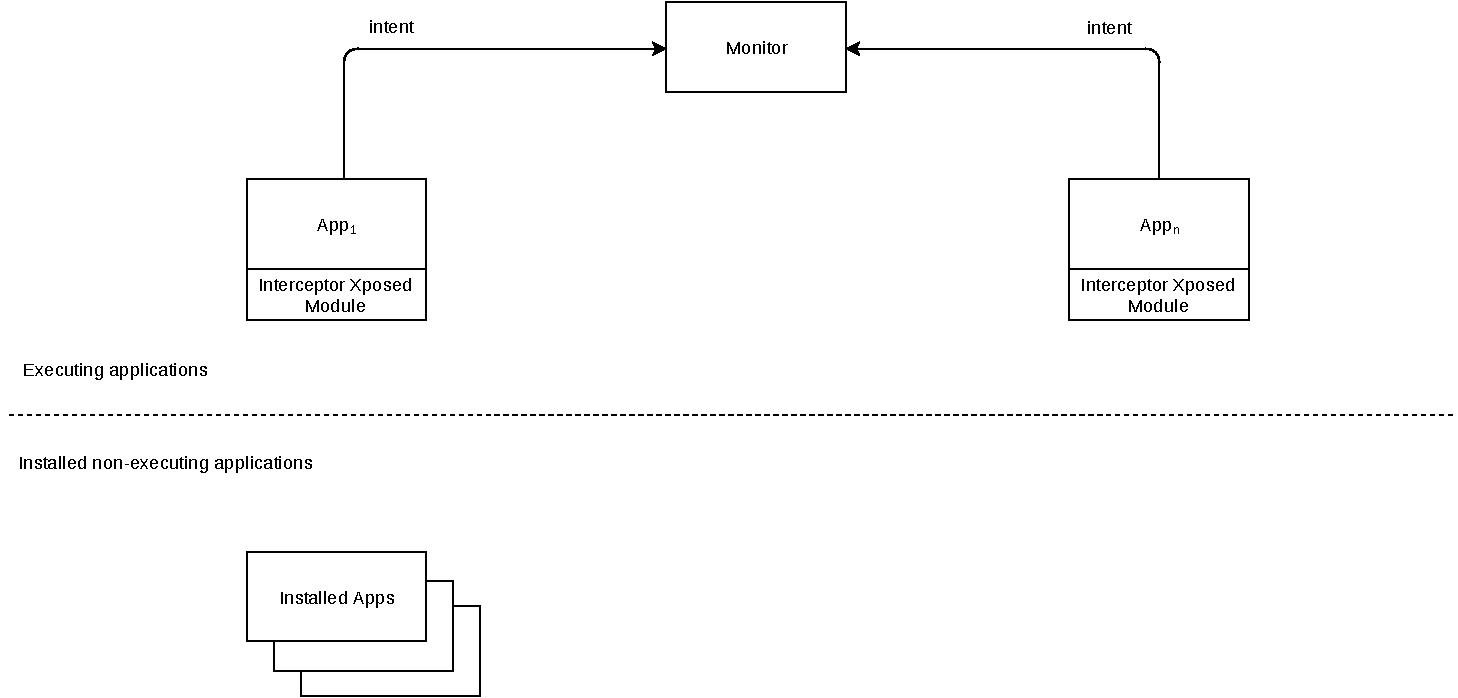
\includegraphics[width=0.7\textwidth]{HighLevelArchitecture.pdf}
\end{center}

Our system architecture (see above) makes use of the Xposed framework \cite{rovo89} in order to intercept calls to security sensitive Android O/S functions.  It adds a monitor app to the user's device which logs these calls and, at arrival of a new event, checks for each security property of interest if it is fulfilled or not.  The security properties are encoded in linear temporal logic (LTL).  In a first attempt we utilised an algorithm by Rosu and Havelund \cite{RosuHavelund} which appeared to be interesting thanks to it's low complexity: for the cost of one evaluation of a property $ \varphi $ is $ O(|t| * |\varphi|) $.  However upon investigation we discovered the dynamic complexity to be $ O(|t|^2 * |\varphi|) $.  This revealed the algorithm to be unsuitable for our requirements.  We made changes that resulted in a new algorithm with a dynamic complexity of $ O(|\varphi|) $.

Related papers

Detection of App Collusion Potential Using Logic Programming.  \cite{PrologAppCollusion}
Runtime verification meets Android security.  \cite{bauer2012runtime}

%[TODO Add some reference to related papers]

%  We define sequences of activity that indicate possible information theft as linear temporal logic formulae and use an algorithm derived from Grigore Rosu and Klaus Havelund to look for those sequences within the activity trace.

%The LTL formula we use to detect collusion between processes engaging in information theft is:

%$ (\square s\ \land (\neg s\ U\ \square q)) \land (\square r \land (\neg r\ U\ \square s)) \land (\square p \land (\neg p\ U\ \square r)) $

@inproceedings{bauer2012runtime,
	title={Runtime verification meets Android security},
	author={Bauer, Andreas and K{\"u}ster, Jan-Christoph and Vegliach, Gil},
	booktitle={NASA Formal Methods Symposium},
	pages={174--180},
	year={2012},
	organization={Springer}
}

@article{PrologAppCollusion,
	author = {Blasco, Jorge and Chen, Thomas and Muttik, Igor and Roggenbach, Markus},
	year = {2017},
	month = {06},
	pages = {},
	title = {Detection of App Collusion Potential Using Logic Programming},
	volume = {105},
	journal = {Journal of Network and Computer Applications},
	doi = {10.1016/j.jnca.2017.12.008}
}

@techreport{RosuHavelund,
	author = {Rosu, Grigore and Havelund, Klaus},
	title = {Synthesizing Dynamic Programming Algorithms from Linear Temporal Logic Formulae},
	year = {2001},
	publisher = {RIACS},
	abstract = {The problem of testing a linear temporal logic (LTL) formula on a finite execution trace of events, generated by an executing program, occurs naturally in runtime analysis of software. We present an algorithm which takes an LTL formula and generates an efficient dynamic programming algorithm. The generated algorithm tests whether the LTL formula is satisfied by a finite trace of events given as input. The generated algorithm runs in linear time, its constant depending on the size of the LTL formula. The memory needed is constant, also depending on the size of the formula.}
}
\end{document}
